\documentclass[11pt,reqno]{amsart}

\usepackage[margin=1in]{geometry}
\usepackage{amsmath,amssymb,amsthm,mathtools}
\usepackage{tikz}
\usepackage[colorlinks=true,linkcolor=blue,citecolor=blue,urlcolor=blue]{hyperref}

\theoremstyle{plain}
\newtheorem{theorem}{Theorem}
\newtheorem{proposition}[theorem]{Proposition}
\newtheorem{lemma}[theorem]{Lemma}
\newtheorem{corollary}[theorem]{Corollary}
\theoremstyle{definition}
\newtheorem{definition}[theorem]{Definition}
\newtheorem{remark}[theorem]{Remark}

\newcommand{\BN}{B_N}
\newcommand{\TN}{T_N}
\newcommand{\Z}{\mathbb{Z}}
\newcommand{\Q}{\mathbb{Q}}
\DeclareMathOperator{\dist}{dist}
\newcommand{\norm}[1]{\left\lVert #1\right\rVert}

\title[Diophantine singularity of shifted KMS matrices]
{Diophantine singularity and conditioning of shifted\\
Kac--Murdock--Szeg\H{o} matrices}

\author{Charlie Dorsey}
\address{Independent researcher, Fort Collins, Colorado, USA}
\email{charliedorsey@gmail.com}

\date{September 2026}

\subjclass[2020]{15A18 (Primary); 15B05, 47B35, 65F35, 11J20, 11J70 (Secondary)}
\keywords{Kac--Murdock--Szeg\H{o} matrix, Toeplitz matrix, condition number,
inhomogeneous Diophantine approximation, singularity, equidistribution, phase quantization}

\hypersetup{
  pdftitle={Diophantine singularity and conditioning of shifted Kac-Murdock-Szego matrices},
  pdfauthor={Charlie Dorsey},
  pdfsubject={Spectral singularity, Diophantine approximation and conditioning of shifted KMS matrices},
  pdfkeywords={Kac-Murdock-Szego, Toeplitz, Diophantine approximation, singularity, condition number}
}

\begin{document}

\begin{abstract}
For $N\ge2$, let $T_N(a)=[a^{|i-j|}]_{i,j=0}^{N-1}$, with $0<a<1$, be the
$N\times N$ Kac--Murdock--Szeg\H{o} matrix, and fix a real level $\tau$.
As the dimension varies, we ask when $\tau$ is an eigenvalue and how ill-conditioned
$T_N(a)-\tau I_N$ becomes when the spectrum nearly hits it.  Outside the range of
the KMS symbol the condition numbers stay uniformly bounded, while at either band
edge they grow quadratically with explicit constants.  Inside the band, the exact
KMS phase law converts the problem to one inhomogeneous Diophantine residual
$d_N=\operatorname{dist}(N\alpha-\beta,\mathbb Z)$ in smooth coordinates
$(\alpha,\beta)$ on an open triangle.

Exact singularity is equivalent to $d_N=0$.  Hence the number of singular
dimensions is always $0$, $1$, or $\infty$; all three behaviors are dense, although
the never-singular parameters have full Lebesgue measure.  At every sufficiently
large nonsingular interior dimension,
$\sigma_{\min}(T_N(a)-\tau I_N)$ is an explicit constant times $d_N/(N+\tau)$,
so the condition number is an explicit constant times $(N+\tau)/d_N$.
Rational $\alpha$ gives periodic behavior.  Irrational $\alpha$ gives an
equidistributed bulk, a Pareto condition-number law of tail index $1$, and rare
spikes controlled by one-sided inhomogeneous approximation.  The hollow case
$\tau=1$ is the resonant diagonal $\beta=\alpha$, where the arithmetic becomes
homogeneous.
\end{abstract}

\maketitle

\section{Introduction}\label{sec:intro}

Fix $0<a<1$ and consider the real symmetric Kac--Murdock--Szeg\H{o} matrix
\begin{equation}\label{eq:Tdef}
T_N(a)=\bigl[a^{|i-j|}\bigr]_{i,j=0}^{N-1},\qquad N\ge2.
\end{equation}
These matrices are classical finite AR$(1)$ correlation matrices.  Fix a real
spectral level $\tau$ and consider the shifted family
\begin{equation}\label{eq:Bdef}
B_N(a,\tau)=T_N(a)-\tau I_N.
\end{equation}
Here $I_N$ is the $N\times N$ identity matrix.  Our question is cross-dimensional: as $N$ varies, when is $\tau$ an eigenvalue of
$T_N(a)$, and how close does the spectrum come when it is not?  Because $B_N$ is
symmetric, this is also a conditioning problem.  Its smallest singular value is the
distance from $\tau$ to the spectrum of $T_N(a)$.  Thus an exact hit makes $B_N$
singular, while a near hit makes it ill-conditioned.  At nonsingular dimensions we
write
\[
\kappa_2(B_N)=\frac{\sigma_{\max}(B_N)}{\sigma_{\min}(B_N)}
\]
for the spectral condition number.

The KMS symbol is the Poisson kernel
\begin{equation}\label{eq:symbol}
\mu_a(\theta)=\frac{1-a^2}{1-2a\cos\theta+a^2},
\qquad 0\le\theta\le\pi,
\end{equation}
strictly decreasing on $(0,\pi)$ with range
\begin{equation}\label{eq:band}
\mu_-(a)=\frac{1-a}{1+a},
\qquad
\mu_+(a)=\frac{1+a}{1-a}.
\end{equation}
These three positions lead to three different mechanisms.  Outside the symbol band
there is a fixed spectral gap.  At a band edge the symbol meets the level
quadratically.  In the interior there is a genuine crossing, and it is here that the
arithmetic enters.

The mechanism can be stated before it is proved.  The finite KMS eigenangles obey
an exact monotone phase law
\[
N\theta+\psi_a(\theta)=k\pi,
\qquad
\psi_a'(\theta)=\mu_a(\theta).
\]
For an interior level $\mu_-(a)<\tau<\mu_+(a)$, let $\theta_\tau$ denote the
unique crossing angle defined by
\begin{equation}\label{eq:crossing}
\mu_a(\theta_\tau)=\tau.
\end{equation}
Set
\begin{equation}\label{eq:alphabeta-intro}
\alpha=\frac{\theta_\tau}{\pi},
\qquad
\beta=1-\frac{\psi_a(\theta_\tau)}{\pi}.
\end{equation}
At the crossing, the phase location is $N\alpha+1-\beta$.  Its distance to the
nearest integer is therefore
\begin{equation}\label{eq:dndef}
d_N=\operatorname{dist}(N\alpha-\beta,\mathbb Z),
\end{equation}
Sections~\ref{sec:kms}--\ref{sec:triangle} show that $(\alpha,\beta)$ are exact
coordinates on the interior parameter region and that this same residual appears in
the determinant.  In particular, $B_N$ is singular exactly when $d_N=0$.  The
cross-dimensional spectral problem is therefore reduced to a single arithmetic
question: how closely does the orbit $N\alpha$ approach the target $\beta$ modulo
one?

To state the conditioning law, define
\begin{equation}\label{eq:gammaC}
\gamma(a,\tau)=|\mu_a'(\theta_\tau)|,
\quad
M(a,\tau)=\max\{\mu_+-\tau,\tau-\mu_-\},
\quad
C(a,\tau)=\frac{M(a,\tau)}{\pi\gamma(a,\tau)}.
\end{equation}
\begin{theorem}[Main conditioning theorem]\label{thm:main-conditioning}
Fix $0<a<1$ and let $N\to\infty$.
\begin{enumerate}
\item If $\tau<\mu_-$, then
\[
\kappa_2(B_N)<\frac{\mu_+-\tau}{\mu_--\tau},
\qquad
\kappa_2(B_N)\longrightarrow\frac{\mu_+-\tau}{\mu_--\tau}.
\]
\item If $\tau=\mu_-$, then
\[
\kappa_2(B_N)
=\frac{4\mu_+^2}{\pi^2}(N+\mu_-)^2\bigl(1+O(N^{-2})\bigr).
\]
\item If $\mu_-<\tau<\mu_+$, then at every sufficiently large nonsingular
$N$,
\[
\sigma_{\min}(B_N)
=\pi\gamma(a,\tau)\frac{d_N}{N+\tau}\bigl(1+O(N^{-1})\bigr),
\qquad
\kappa_2(B_N)
=C(a,\tau)\frac{N+\tau}{d_N}\bigl(1+O(N^{-1})\bigr).
\]
\item If $\tau=\mu_+$, then
\[
\kappa_2(B_N)
=\frac{4\mu_-^2}{\pi^2}(N+\mu_+)^2\bigl(1+O(N^{-2})\bigr).
\]
\item If $\tau>\mu_+$, then
\[
\kappa_2(B_N)<\frac{\tau-\mu_-}{\tau-\mu_+},
\qquad
\kappa_2(B_N)\longrightarrow\frac{\tau-\mu_-}{\tau-\mu_+}.
\]
\end{enumerate}
The interior error terms are for fixed $(a,\tau)$; they are not uniform as
$\tau$ approaches a band edge.
\end{theorem}

The theorem cleanly separates analysis from arithmetic.  Outside the band,
conditioning stays bounded; at either edge it grows quadratically.  In the interior,
all irregularity is concentrated in the scalar sequence $d_N$.  For rational
$\alpha$, this sequence is periodic, and exact singularity is either absent or
recurrent on one residue class.  For irrational $\alpha$, at most one exact singular
dimension can occur; equidistribution governs the bulk, while unusually small values
of $d_N$ produce exceptional conditioning spikes.  Consequently the number of
singular dimensions is always $0$, $1$, or $\infty$.

The special shift $\tau=1$, for which $B_N=T_N-I_N$ has zero diagonal, is not a
separate mechanism.  In the coordinates above it is the diagonal $\beta=\alpha$,
the $N=1$ member of the same affine singularity web.  There the residual becomes
$\operatorname{dist}((N-1)\alpha,\mathbb Z)$, so the inhomogeneous problem reduces
to homogeneous approximation.  We return to this hollow resonance only after the
general shifted problem is in place.

The classical inputs and the contribution claimed here should be kept distinct.
KMS spectral formulas, characteristic-polynomial recurrences, Toeplitz phase
methods, and the Diophantine approximation theorems used later all have substantial
prior literature
\cite{KMS,GrenanderSzego,ChremmosFikioris2016,Fikioris2018,BBGM2015,BBGM2016,
DaviesLevitin2014,BogoyaEtAl2026}.  What is claimed here is the KMS-specific
fixed-level dictionary: explicit interior coordinates, the affine residual
$N\alpha-\beta$, an exact singularity classification, a determinant formula organized
around that residual, and the resulting conditioning laws with explicit leading
constants.  Section~\ref{sec:scope} states the detailed prior-art boundary.

The paper follows that dictionary in dependency order.  Section~\ref{sec:kms}
puts the classical KMS spectrum into the exact monotone phase form needed here.
Section~\ref{sec:triangle} converts a fixed interior level into the coordinates
$(\alpha,\beta)$ and derives the determinant formula.  Section~\ref{sec:singularity}
classifies exact singularity and recurrence.  Section~\ref{sec:conditioning}
proves the five conditioning regimes.  Section~\ref{sec:dioph} then reads the
interior formula through rational periodicity, irrational equidistribution, and
one-sided inhomogeneous approximation.  Section~\ref{sec:resonance} recovers the
hollow case as a resonant slice of the same geometry.

\section{KMS quantization and Blaschke phase}\label{sec:kms}
Two spectral facts drive everything that follows: the eigenangles are level sets of
one strictly increasing phase, and the derivative of that phase is
$N+\mu_a(\theta)$.  This section derives both facts from the classical KMS
recurrence.  It also records the disk-automorphism form of the boundary phase, which
makes the identity $\psi_a'=\mu_a$ transparent.

Throughout the rest of the paper we use
\[
\mu_a(\theta)=\frac{1-a^2}{1-2a\cos\theta+a^2},
\qquad
\mu_- = \frac{1-a}{1+a},
\qquad
\mu_+ = \frac{1+a}{1-a}.
\]
Thus $\mu_-\le\mu_a(\theta)\le\mu_+$ on $[0,\pi]$.

The inverse of \eqref{eq:Tdef} is
\begin{equation}\label{eq:Tinv}
T_N(a)^{-1}=\frac1{1-a^2}
\begin{pmatrix}
1 & -a \\
-a & 1+a^2 & -a\\
& \ddots & \ddots & \ddots\\
&&-a&1+a^2&-a\\
&&&-a&1
\end{pmatrix};
\end{equation}
see \cite{KMS}.  The corresponding second-order recurrence gives the standard
secular function
\begin{equation}\label{eq:secular}
S_N(\theta)
=\sin((N+1)\theta)-2a\sin(N\theta)+a^2\sin((N-1)\theta).
\end{equation}
Define
\begin{equation}\label{eq:DE}
D(\theta)=(1+a^2)\cos\theta-2a,
\qquad
E(\theta)=(1-a^2)\sin\theta,
\end{equation}
and, for $0<\theta<\pi$,
\begin{equation}\label{eq:psi}
\psi_a(\theta)=\arg(D(\theta)+iE(\theta))\in(0,\pi).
\end{equation}
Put
\[
R(\theta)=\sqrt{D(\theta)^2+E(\theta)^2}
=1-2a\cos\theta+a^2.
\]

\begin{lemma}[Phase form]\label{lem:phase}
For $0<\theta<\pi$,
\begin{equation}\label{eq:phaseform}
S_N(\theta)=R(\theta)\sin\bigl(N\theta+\psi_a(\theta)\bigr).
\end{equation}
Moreover $\psi_a$ extends continuously to $[0,\pi]$ with
$\psi_a(0)=0$ and $\psi_a(\pi)=\pi$.
\end{lemma}

\begin{proof}
Expanding the outer sine terms in \eqref{eq:secular} gives
\[
S_N(\theta)=D(\theta)\sin(N\theta)+E(\theta)\cos(N\theta),
\]
which is \eqref{eq:phaseform}.  At the endpoints $E$ vanishes while
$D(0)=(1-a)^2>0$ and $D(\pi)=-(1+a)^2<0$.
\end{proof}

\begin{proposition}[Disk-automorphism form of the phase]\label{prop:blaschke}
Let
\begin{equation}\label{eq:blaschke}
b_a(z)=\frac{z-a}{1-az}.
\end{equation}
For $0<\theta<\pi$,
\begin{equation}\label{eq:blaschkephase}
\boxed{
e^{i\psi_a(\theta)}=b_a(e^{i\theta}).}
\end{equation}
Consequently
\begin{equation}\label{eq:psiprime}
\boxed{
\psi_a'(\theta)=
\frac{1-a^2}{|1-ae^{i\theta}|^2}
=\mu_a(\theta).}
\end{equation}
At every eigenangle $\theta_k$, with $z_k=e^{i\theta_k}$,
\begin{equation}\label{eq:blaschkequant}
\boxed{z_k^N b_a(z_k)=(-1)^k.}
\end{equation}
\end{proposition}

\begin{proof}
There is an exact factorization
\[
D(\theta)+iE(\theta)
=e^{-i\theta}(e^{i\theta}-a)^2.
\]
Since
\[
|e^{i\theta}-a|^2
=(e^{i\theta}-a)(e^{-i\theta}-a),
\]
dividing by the modulus gives
\[
\frac{D+iE}{|D+iE|}
=\frac{e^{i\theta}-a}{1-ae^{i\theta}},
\]
which is \eqref{eq:blaschkephase}.  The angular derivative of the boundary
argument of the disk automorphism $b_a$ is the Poisson kernel,
\[
\frac{d}{d\theta}\arg b_a(e^{i\theta})
=\frac{1-a^2}{|1-ae^{i\theta}|^2},
\]
giving \eqref{eq:psiprime}.  Finally, the exact phase quantization below is
$N\theta_k+\psi_a(\theta_k)=k\pi$; exponentiation gives
\eqref{eq:blaschkequant}.
\end{proof}

\begin{remark}
The use of Blaschke boundary phases and Pr\"ufer-type arguments in zero-spacing
problems is classical; see, for example, Simanek \cite{Simanek2020}.  Likewise,
finite Bernstein--Szeg\H{o} Jacobi systems admit exact phase equations built from
finite products of Möbius factors \cite{vanDiejenEmsiz2018}.  Proposition
\ref{prop:blaschke} is recorded because in the KMS family the same Poisson kernel
is simultaneously the spectral symbol, which is what later turns the generic local
factor $N+\psi_a'(\theta_\tau)$ into $N+\tau$.
\end{remark}

Set
\begin{equation}\label{eq:G}
G_N(\theta)=N\theta+\psi_a(\theta).
\end{equation}
Then
\begin{equation}\label{eq:Gprime}
G_N'(\theta)=N+\mu_a(\theta)>0.
\end{equation}

\begin{theorem}[Exact quantization]\label{thm:quant}
The $N$ KMS eigenangles are the unique points
\[
0<\theta_1<\cdots<\theta_N<\pi
\]
satisfying
\begin{equation}\label{eq:quant}
G_N(\theta_k)=k\pi,
\qquad k=1,\ldots,N.
\end{equation}
They are simple and obey
\begin{equation}\label{eq:spacing}
\frac{\pi}{N+\mu_+}
\le \theta_{k+1}-\theta_k
\le \frac{\pi}{N+\mu_-}.
\end{equation}
The corresponding KMS eigenvalues and eigenvectors are
\begin{equation}\label{eq:eigs}
\mu_k=\mu_a(\theta_k),
\qquad
v_j^{(k)}=\sin((j+1)\theta_k)-a\sin(j\theta_k),
\quad j=0,\ldots,N-1.
\end{equation}
Hence the eigenvalues of $B_N(a,\tau)$ are
\begin{equation}\label{eq:shiftedeigs}
\lambda_k(a,\tau)=\mu_a(\theta_k)-\tau.
\end{equation}
\end{theorem}

\begin{proof}
By Lemma~\ref{lem:phase}, the roots of the secular equation are the preimages of
$\pi\mathbb Z$ under $G_N$.  Equation \eqref{eq:Gprime} shows that $G_N$
increases from $0$ to $(N+1)\pi$, giving exactly \eqref{eq:quant}.  The spacing
estimate follows from the mean-value theorem and
$\mu_-\le\mu_a\le\mu_+$.  The eigenvalue and eigenvector formulas are the
standard solution of the recurrence from \eqref{eq:Tinv}; see also
\cite{Fikioris2018,BBGM2015,BBGM2016}.  Subtracting $\tau I_N$ shifts the
eigenvalues without changing the eigenvectors.
\end{proof}

\section{The Diophantine triangle and the determinant}\label{sec:triangle}

The phase law locates every finite eigenangle.  For a fixed spectral level, we now
freeze the crossing angle and record its position relative to that phase grid.  Two
steps are needed: identify the original parameter region in coordinates
$(\alpha,\beta)$, then show that the same affine residual $N\alpha-\beta$ appears in
the characteristic polynomial.

Assume throughout this section that
\begin{equation}\label{eq:interior}
\mu_-(a)<\tau<\mu_+(a).
\end{equation}
There is a unique $\theta_\tau\in(0,\pi)$ satisfying \eqref{eq:crossing}, with
\begin{equation}\label{eq:costheta}
\cos\theta_\tau
=\frac{1+a^2-(1-a^2)/\tau}{2a}.
\end{equation}
Define
\begin{equation}\label{eq:alphabeta}
\alpha=\frac{\theta_\tau}{\pi},
\qquad
\beta=1-\frac{\psi_a(\theta_\tau)}{\pi}.
\end{equation}

\begin{theorem}[Diophantine-triangle coordinates]\label{thm:triangle}
The map $(a,\tau)\mapsto(\alpha,\beta)$ is a bijection from the interior parameter
region
\[
\{(a,\tau):0<a<1,\ \mu_-(a)<\tau<\mu_+(a)\}
\]
onto the open triangle
\begin{equation}\label{eq:triangle}
\mathcal D=\{(\alpha,\beta):\alpha>0,\ \beta>0,\ \alpha+\beta<1\}.
\end{equation}
The inverse is
\begin{equation}\label{eq:inverse}
\boxed{
\tau=\frac{\sin(\pi\beta)}{\sin(\pi\alpha)},
\qquad
 a=\frac{\cos\frac\pi2(\alpha+\beta)}
         {\cos\frac\pi2(\alpha-\beta)}.}
\end{equation}
\end{theorem}

\begin{proof}
For a general interior angle $\theta$, write $\psi=\psi_a(\theta)$ and
$D+iE=Re^{i\psi}$.  Then
\[
R\sin(\psi-\theta)=E\cos\theta-D\sin\theta
=2a(1-a\cos\theta)\sin\theta>0.
\]
Since $0<\theta,\psi<\pi$, this gives
\[
0<\theta<\psi<\pi.
\]
At the crossing, $\theta=\pi\alpha$ and $\psi=\pi(1-\beta)$, hence
$\alpha>0$, $\beta>0$ and $\alpha+\beta<1$.

Next, $E=R\sin\psi=(1-a^2)\sin\theta$, while
$\tau=(1-a^2)/R$ at the crossing.  Thus
\[
\tau=\frac{\sin\psi}{\sin\theta}
=\frac{\sin(\pi\beta)}{\sin(\pi\alpha)}.
\]
For the formula for $a$, observe the exact factorization
\begin{equation}\label{eq:factor}
D+iE=e^{-i\theta}(e^{i\theta}-a)^2.
\end{equation}
If $\gamma=\arg(e^{i\theta}-a)$, then $\psi=2\gamma-\theta$ and therefore
$\gamma=(\psi+\theta)/2$.  Resolving the triangle formed by
$e^{i\theta}-a$ gives
\[
a=\frac{\sin\frac12(\psi-\theta)}
        {\sin\frac12(\psi+\theta)}
 =\frac{\cos\frac\pi2(\alpha+\beta)}
        {\cos\frac\pi2(\alpha-\beta)}.
\]
Conversely, let $(\alpha,\beta)$ satisfy \eqref{eq:triangle} and put
$\theta=\pi\alpha$, $\psi=\pi(1-\beta)$ and
$\gamma=(\theta+\psi)/2$.  Then $0<\theta<\psi<\pi$.  Formula
\eqref{eq:inverse} gives
\[
a=\frac{\sin(\gamma-\theta)}{\sin\gamma},
\]
so $0<a<1$ (equivalently, in the cosine form of \eqref{eq:inverse}, the numerator
and denominator are positive and the numerator is smaller).  Moreover
\[
e^{i\theta}-a=\frac{\sin\theta}{\sin\gamma}e^{i\gamma}.
\]
Using \eqref{eq:factor}, the corresponding boundary phase is therefore
$2\gamma-\theta=\psi$.  Since
$E=R\sin\psi=(1-a^2)\sin\theta$, we obtain
\[
\mu_a(\theta)=\frac{1-a^2}{R}
=\frac{\sin\psi}{\sin\theta}
=\frac{\sin(\pi\beta)}{\sin(\pi\alpha)}=\tau.
\]
Thus $\theta$ is the crossing angle and the constructed pair maps back to
$(\alpha,\beta)$, proving surjectivity and uniqueness.
\end{proof}

The coordinate theorem locates the fixed level in phase space.  Exact singularity,
however, is a statement about the characteristic polynomial at that same level.
The following shifted Chebyshev form supplies the bridge.  It is recorded here in a
self-contained form and is equivalent to classical KMS characteristic-polynomial
formulas; see \cite{Fikioris2018}.

The determinant recurrence itself is classical.  Chremmos and Fikioris derive a
second-order recurrence for the characteristic polynomial of the same geometric
Toeplitz family \cite{ChremmosFikioris2016}; under the real KMS specialization, that
machinery contains the hollow ($\tau=1$) determinant identity.  We use the
inverse/Chebyshev route below because it places the general scalar shift directly in
the $(a,\tau)$ variables needed for the fixed-level problem.

\begin{lemma}[Shifted Chebyshev determinant]\label{lem:chebshift}
For $N\ge2$, $0<a<1$, and $\tau\ne0$,
\begin{equation}\label{eq:chebshift}
\det(\TN(a)-\tau I_N)
=\frac{(\tau a)^N}{1-a^2}
\bigl[U_N(x)+2aU_{N-1}(x)+a^2U_{N-2}(x)\bigr],
\end{equation}
where $U_j$ is the Chebyshev polynomial of the second kind and
\begin{equation}\label{eq:xdef}
x=\frac{1-a^2-\tau(1+a^2)}{2\tau a}.
\end{equation}
\end{lemma}

\begin{proof}
The classical KMS inverse is
\[
\TN(a)^{-1}=\frac1{1-a^2}
\begin{pmatrix}
1&-a&&&\\
-a&1+a^2&-a&&\\
&\ddots&\ddots&\ddots&\\
&&-a&1+a^2&-a\\
&&&-a&1
\end{pmatrix},
\qquad
\det\TN(a)=(1-a^2)^{N-1}.
\]
Hence
\[
\det(\TN-\tau I_N)=\frac{\det H_N}{1-a^2},
\]
where $H_N$ is tridiagonal with off-diagonal $b=\tau a$, interior diagonal
$c=1-a^2-\tau(1+a^2)=2bx$, and corner diagonal
$d=1-a^2-\tau=b(2x+a)$.
Let $P_k$ be the determinant of the leading $k\times k$ block before the final
corner modification.  Then
\[
P_0=1,\qquad P_1=d,\qquad P_k=cP_{k-1}-b^2P_{k-2},
\]
so, with $U_{-1}=0$,
\[
P_k=b^k\bigl(U_k(x)+aU_{k-1}(x)\bigr).
\]
Applying the last corner gives
\[
\det H_N=dP_{N-1}-b^2P_{N-2}
=b^N\bigl(U_N(x)+2aU_{N-1}(x)+a^2U_{N-2}(x)\bigr),
\]
by the Chebyshev recurrence $U_j=2xU_{j-1}-U_{j-2}$.  This proves
\eqref{eq:chebshift}.
\end{proof}

For $x\in\mathbb R$, write $\norm{x}=\dist(x,\mathbb Z)$ for distance to the
nearest integer.

\begin{theorem}[Exact determinant]\label{thm:det}
For every interior pair $(a,\tau)$ and every $N\ge2$,
\begin{equation}\label{eq:det}
\boxed{
\det\BN(a,\tau)
=(-1)^{N+1}a^N\tau^{N-1}
\frac{\sin\pi(N\alpha-\beta)}{\sin(\pi\alpha)}.}
\end{equation}
Consequently, with
\begin{equation}\label{eq:dN}
d_N=\norm{N\alpha-\beta}=\dist(N\alpha-\beta,\Z),
\end{equation}
\begin{equation}\label{eq:detdepth}
|\det\BN(a,\tau)|
=a^N\tau^{N-1}
\frac{\sin(\pi d_N)}{\sin(\pi\alpha)}.
\end{equation}
\end{theorem}

\begin{proof}
At the crossing, \eqref{eq:costheta} implies $x=-\cos\theta_\tau$.  Since
$U_j(-\cos\theta)=(-1)^j\sin((j+1)\theta)/\sin\theta$, the bracket in
\eqref{eq:chebshift} becomes
\[
(-1)^N\frac{S_N(\theta_\tau)}{\sin\theta_\tau}.
\]
By Lemma~\ref{lem:phase},
\[
S_N(\theta_\tau)
=R(\theta_\tau)\sin(N\theta_\tau+\psi_a(\theta_\tau)).
\]
Since $R(\theta_\tau)=(1-a^2)/\tau$,
$\theta_\tau=\pi\alpha$, and
$\psi_a(\theta_\tau)=\pi(1-\beta)$, substitution into
\eqref{eq:chebshift} yields \eqref{eq:det}.  Taking absolute values and reducing the
sine modulo integers gives \eqref{eq:detdepth}.
\end{proof}

\section{Exact singularity geometry and recurrence}\label{sec:singularity}

The determinant formula reduces exact singularity to one affine arithmetic equation.
We classify that equation before returning to conditioning.  The decisive split is
rational versus irrational $\alpha$: rational phase points can recur periodically,
whereas an irrational phase point can lie on the singularity web at most once.

\begin{theorem}[Exact singularity]\label{thm:sing}
For an interior parameter pair,
\begin{equation}\label{eq:sing}
\boxed{
\BN(a,\tau)\text{ is singular}
\quad\Longleftrightarrow\quad
N\alpha-\beta\in\Z.}
\end{equation}
At a singular dimension the nullity is exactly one.
\end{theorem}

\begin{proof}
The criterion follows from Theorem~\ref{thm:det}.  Simplicity follows from the
simple KMS spectrum in Theorem~\ref{thm:quant}.
\end{proof}

The geometry of \eqref{eq:sing} is the family of affine lines
\begin{equation}\label{eq:web}
\beta=N\alpha-m,
\qquad m\in\Z.
\end{equation}
We refer to their intersections with $\mathcal D$ as the \emph{affine singularity
web}.

\begin{figure}[t]
\centering
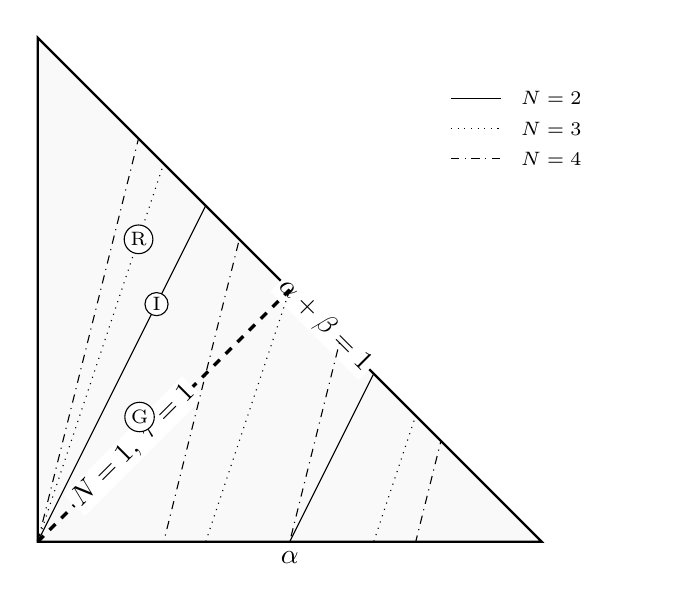
\begin{tikzpicture}[scale=6.4]
  \clip (-0.02,-0.08) rectangle (1.24,1.02);
  \fill[gray!5] (0,0)--(1,0)--(0,1)--cycle;
  \draw[thick] (0,0)--(1,0)--(0,1)--cycle;
  \node[below] at (0.50,0) {$\alpha$};
  \node[left] at (0,0.50) {$\beta$};
  \node[rotate=-45,fill=white,inner sep=1pt] at (0.57,0.43) {$\alpha+\beta=1$};

  % virtual N=1 line
  \draw[very thick,dashed] (0,0)--(0.5,0.5);
  \node[rotate=45,fill=white,inner sep=1pt] at (0.19,0.19)
    {$N=1,\;\tau=1$};

  % physical web lines, genuinely clipped to the target triangle
  \begin{scope}
    \clip (0,0)--(1,0)--(0,1)--cycle;
    \foreach \m in {0,1,2} {
      \draw[thin] plot[domain=0:1,samples=2] (\x,{2*\x-\m});
    }
    \foreach \m in {0,1,2,3} {
      \draw[thin,dotted] plot[domain=0:1,samples=2] (\x,{3*\x-\m});
    }
    \foreach \m in {0,1,2,3,4} {
      \draw[thin,dash dot] plot[domain=0:1,samples=2] (\x,{4*\x-\m});
    }
  \end{scope}

  % representative points: R rational recurrent; I irrational with N=2 hit;
  % G irrational and off the displayed affine web
  \node[draw,circle,fill=white,inner sep=1pt,font=\scriptsize] at (0.20,0.60) {R};
  \node[draw,circle,fill=white,inner sep=1pt,font=\scriptsize]
    at ({sqrt(2)/6},{sqrt(2)/3}) {I};
  \node[draw,circle,fill=white,inner sep=1pt,font=\scriptsize]
    at ({sqrt(2)/7},{sqrt(3)/7}) {G};

  % line-style key
  \draw (0.82,0.88)--(0.92,0.88); \node[anchor=west,font=\scriptsize] at (0.94,0.88) {$N=2$};
  \draw[dotted] (0.82,0.82)--(0.92,0.82); \node[anchor=west,font=\scriptsize] at (0.94,0.82) {$N=3$};
  \draw[dash dot] (0.82,0.76)--(0.92,0.76); \node[anchor=west,font=\scriptsize] at (0.94,0.76) {$N=4$};
\end{tikzpicture}
\caption{The Diophantine target triangle
$\alpha>0$, $\beta>0$, $\alpha+\beta<1$.  Exact singularity at dimension $N$ lies
on the affine lines $\beta\equiv N\alpha\pmod1$; representative lines for
$N=2,3,4$ are shown.  The dashed diagonal is the $N=1$ member of the web, just
outside our nontrivial matrix range, and hence the resonant shift $\tau=1$.  The marked points illustrate a rational recurrent point
(R), an irrational point with one exact physical hit (I), and a generic off-web
point (G).  Theorem~\ref{thm:dense-strata} shows that all three behaviors
are dense in the full triangle, although the off-web, never-singular stratum has
full two-dimensional measure.}
\label{fig:triangle}
\end{figure}


For rational $\alpha$, the web condition becomes a finite congruence problem.

\begin{theorem}[Rational recurrence]\label{thm:rational}
Let $\alpha=p/q$ in lowest terms.
Then singularity occurs for some dimension if and only if
\begin{equation}\label{eq:compat}
q\beta\in\Z.
\end{equation}
If $r=q\beta\in\Z$, then $0<r<q-p$ and the singular dimensions are exactly the one
congruence class
\begin{equation}\label{eq:congruence}
Np\equiv r\pmod q.
\end{equation}
If $q\beta\notin\Z$, there are no singular dimensions.
\end{theorem}

\begin{proof}
The condition $N p/q-\beta\in\Z$ implies $Np-q\beta\in q\Z$, so a solution requires
$q\beta\in\Z$.  Conversely, if $r=q\beta$ is an integer, then the criterion is
\eqref{eq:congruence}.  Since $p$ is invertible mod $q$, this determines exactly one
residue class.  The triangle inequalities imply $0<r<q-p$.
\end{proof}

\begin{corollary}[Complete recurrent parametrization]\label{cor:param}
Every interior parameter pair with infinitely many singular dimensions is obtained
from integers
\[
0<p,
\qquad 0<r,
\qquad p+r<q,
\qquad \gcd(p,q)=1,
\]
by
\begin{equation}\label{eq:param}
\boxed{
\alpha=\frac pq,
\qquad
\beta=\frac rq,
\qquad
\tau=\frac{\sin(r\pi/q)}{\sin(p\pi/q)},
\qquad
 a=\frac{\cos((p+r)\pi/(2q))}
         {\cos((p-r)\pi/(2q))}.}
\end{equation}
The singular dimensions satisfy $Np\equiv r\pmod q$.
\end{corollary}

\subsection*{A recurrent non-hollow family}
Take
\[
\alpha=\frac15,
\qquad
\beta=\frac35.
\]
Then $\alpha+\beta=4/5<1$, and Corollary~\ref{cor:param} gives
\[
a=\frac{\cos(2\pi/5)}{\cos(\pi/5)}
=\frac{3-\sqrt5}{2},
\qquad
\tau=\frac{\sin(3\pi/5)}{\sin(\pi/5)}
=\frac{1+\sqrt5}{2}.
\]
The singularity congruence is
\[
N\equiv3\pmod5.
\]
Thus the same non-hollow eigenvalue $\tau=\varphi$ recurs at every dimension
$N\equiv3\pmod5$ for the KMS decay parameter $a=(3-\sqrt5)/2$.


The rational case permits periodic return.  Irrational $\alpha$ behaves in the
opposite way: two exact hits would force a rational relation.

\begin{theorem}[Irrational uniqueness and the $0/1/\infty$ law]\label{thm:zeroinf}
If $\alpha$ is irrational, $\BN(a,\tau)$ is singular for at most one dimension.
Consequently, for every interior parameter pair,
\begin{equation}\label{eq:card}
\boxed{
\#\{N\ge2:\BN(a,\tau)\text{ singular}\}\in\{0,1,\infty\}.}
\end{equation}
\end{theorem}

\begin{proof}
If two distinct dimensions $N_1,N_2$ were singular, then
\[
N_1\alpha-\beta=m_1,
\qquad
N_2\alpha-\beta=m_2
\]
for integers $m_1,m_2$.  Subtraction gives
$(N_1-N_2)\alpha=m_1-m_2\in\Z$, forcing $\alpha\in\Q$.  The classification now
follows from Theorem~\ref{thm:rational}.
\end{proof}

Cardinality alone does not describe how these three behaviors sit in parameter
space.  The next theorem records both their topological abundance and their measure.

\begin{theorem}[Dense singularity stratification]\label{thm:dense-strata}
For $j\in\{0,1,\infty\}$ define
\[
\mathcal S_j=\left\{(\alpha,\beta)\in\mathcal D:
\#\{N\ge2:B_N(a,\tau)\text{ is singular}\}=j\right\},
\]
where $(a,\tau)$ is the parameter pair corresponding to $(\alpha,\beta)$ through
Theorem~\ref{thm:triangle}.  Then $\mathcal S_0$, $\mathcal S_1$ and
$\mathcal S_\infty$ are all dense in $\mathcal D$.  Moreover,
\begin{enumerate}
\item $\mathcal S_0$ has full two-dimensional Lebesgue measure in $\mathcal D$;
\item $\mathcal S_1$ is uncountable and has two-dimensional measure zero;
\item $\mathcal S_\infty$ is countable and has two-dimensional measure zero.
\end{enumerate}
The same statements hold in the physical interior parameter region
\[
\mathcal P=\{(a,\tau):0<a<1,\ \mu_-(a)<\tau<\mu_+(a)\}.
\]
In particular, arbitrarily close to every interior shifted KMS matrix is one that is
never singular, one that is singular exactly once, and one that is singular infinitely
often, yet almost every interior parameter pair is never exactly singular.
\end{theorem}

\begin{proof}
Let
\[
\mathcal W=\bigcup_{N\ge2}\ \bigcup_{m\in\Z}
\bigl\{(\alpha,\beta)\in\mathcal D:\beta=N\alpha-m\bigr\}
\]
be the affine singularity web.  It is a countable union of line segments and hence
has two-dimensional measure zero.  By Theorem~\ref{thm:sing},
$\mathcal S_0=\mathcal D\setminus\mathcal W$, so $\mathcal S_0$ has full measure;
it is dense because every nonempty open subset of $\mathcal D$ has positive area.

The recurrent set $\mathcal S_\infty$ is countable by Theorem~\ref{thm:rational}.
It is dense: given $(\alpha_0,\beta_0)\in\mathcal D$, choose arbitrarily large
primes $q$ and integers $p,r$ with
\[
\frac pq\to\alpha_0,
\qquad
\frac rq\to\beta_0,
\qquad
p+r<q.
\]
For large $q$ one has $1\le p\le q-1$, so $\gcd(p,q)=1$, while
$q(r/q)=r\in\Z$; Theorem~\ref{thm:rational} therefore places
$(p/q,r/q)$ in $\mathcal S_\infty$.

Finally, $\mathcal S_1=\mathcal W\setminus\mathcal S_\infty$.  Indeed, a point of
$\mathcal W$ with irrational $\alpha$ has exactly one hit by
Theorem~\ref{thm:zeroinf}, whereas a point of $\mathcal W$ with rational $\alpha$
is automatically compatible and hence recurrent by Theorem~\ref{thm:rational}.
Thus $\mathcal S_1$ has measure zero.  It is uncountable, and it is dense because
through every recurrent point passes a web segment containing irrational-$\alpha$
points arbitrarily nearby; the density of $\mathcal S_\infty$ then gives the claim.

The map of Theorem~\ref{thm:triangle} is a smooth bijection with smooth inverse on
the two open interiors.  It therefore preserves density and cardinality, and,
locally on compact subsets, preserves null sets in both directions.  The same
stratification statements consequently hold in $\mathcal P$.
\end{proof}


\subsection*{Further exact spectral consequences}

The next two consequences are not needed for conditioning, but they complete the
fixed-level spectral picture.  Write $n_+(A)$ for the number of positive eigenvalues
of a real symmetric matrix $A$, counted with multiplicity.  Quantization makes the
inertia immediate: a shifted eigenvalue is positive exactly when
$\theta_k<\theta_\tau$.

\begin{proposition}[Inertia staircase]\label{prop:inertia}
For every interior parameter pair and $N\ge2$,
\begin{equation}\label{eq:inertia}
\boxed{
n_+(\BN(a,\tau))=\left\lceil N\alpha-\beta\right\rceil.}
\end{equation}
If $N\alpha-\beta\in\Z$, exactly one eigenvalue is zero; otherwise none is zero.
The number of negative eigenvalues is the remainder.
\end{proposition}

\begin{proof}
By monotonicity of $\mu_a$, $\lambda_k>0$ iff $\theta_k<\theta_\tau$.  Since $G_N$
is increasing, this is equivalent to
\[
k\pi<G_N(\theta_\tau)
=\pi(N\alpha+1-\beta).
\]
Counting integers $1\le k\le N$ below this threshold gives
$\lceil N\alpha-\beta\rceil$.  Equality in the threshold is exactly the singularity
criterion.
\end{proof}

\begin{proposition}[Kernel]\label{prop:kernel}
At a singular dimension,
\begin{equation}\label{eq:kernel}
\ker\BN(a,\tau)
=\operatorname{span}\left\{
\bigl(\sin((j+1)\theta_\tau)-a\sin(j\theta_\tau)\bigr)_{j=0}^{N-1}
\right\}.
\end{equation}
\end{proposition}

\begin{proof}
Evaluate the eigenvector formula \eqref{eq:eigs} at the crossing angle, which is an
eigenangle precisely at singularity.  Nullity one was proved in
Theorem~\ref{thm:sing}.
\end{proof}

\section{Conditioning across the symbol band}\label{sec:conditioning}

The three positions relative to the symbol band now produce three local mechanisms.
At an interior crossing the symbol has nonzero slope, so phase error converts
linearly into spectral error.  At either edge that slope vanishes and the first
nonzero term is quadratic.  Outside the band there is no crossing and a fixed gap
remains.  We treat the interior first, then the exterior and edge cases.

All interior asymptotic statements in this section are for a fixed pair
$(a,\tau)$ with $\mu_-<\tau<\mu_+$; implied constants may depend on that pair.
We first treat the interior band.  Put
\begin{equation}\label{eq:gamma}
\gamma(a,\tau)=|\mu_a'(\theta_\tau)|.
\end{equation}
A direct substitution into the derivative of \eqref{eq:symbol} gives
\begin{equation}\label{eq:gamma-form}
\boxed{
\gamma(a,\tau)
=\frac{2a\tau^2\sin(\pi\alpha)}{1-a^2}.}
\end{equation}
Equivalently, differentiating
$\mu(\theta)=\sin\psi_a(\theta)/\sin\theta$ and using $\psi_a'=\mu_a$ gives
\begin{equation}\label{eq:gamma-phase}
\gamma(a,\tau)
=\tau\bigl(\cot(\pi\alpha)-\tau\cot(\pi(1-\beta))\bigr),
\end{equation}
with the sign understood through the absolute value in \eqref{eq:gamma}.

The interior proof has two steps.  First locate the eigenangle whose phase index is
nearest the fixed crossing; then pass from angular displacement to spectral
displacement through the slope $\gamma(a,\tau)$.

For sufficiently large $N$, the nearest integer to
$G_N(\theta_\tau)/\pi=N\alpha+1-\beta$ belongs to the physical index set
$\{1,\ldots,N\}$.  Choose such a nearest integer $k_N$.

\begin{theorem}[Nonasymptotic localization]\label{thm:localization}
For all sufficiently large $N$,
\begin{equation}\label{eq:localization}
\frac{\pi d_N}{N+\mu_+}
\le
|\theta_{k_N}-\theta_\tau|
\le
\frac{\pi d_N}{N+\mu_-}.
\end{equation}
For nonsingular dimensions,
\begin{equation}\label{eq:local-asymp}
\boxed{
|\theta_{k_N}-\theta_\tau|
=\frac{\pi d_N}{N+\tau}\bigl(1+O(N^{-2})\bigr).}
\end{equation}
\end{theorem}

\begin{proof}
The distance from $G_N(\theta_\tau)$ to the nearest multiple of $\pi$ is exactly
$\pi d_N$.  The mean-value theorem and
$N+\mu_-\le G_N'\le N+\mu_+$ yield \eqref{eq:localization}.  Hence the intermediate
point lies $O(N^{-1})$ from $\theta_\tau$, so
$\mu_a(\xi)=\tau+O(N^{-1})$.  Thus
\[
N+\mu_a(\xi)=N+\tau+O(N^{-1}),
\]
a relative $O(N^{-2})$ perturbation of $N+\tau$, giving
\eqref{eq:local-asymp}.
\end{proof}

The preceding theorem is a phase-space estimate.  Because the crossing is interior,
$|\mu_a'(\theta_\tau)|=\gamma(a,\tau)>0$, so it now translates directly into the
smallest singular value.

\begin{theorem}[Interior smallest singular value]\label{thm:smin}
For every fixed interior pair and every sufficiently large nonsingular dimension,
\begin{equation}\label{eq:smin}
\boxed{
\sigma_{\min}(\BN(a,\tau))
=\pi\gamma(a,\tau)\frac{d_N}{N+\tau}
\bigl(1+O(N^{-1})\bigr).}
\end{equation}
At an exact singular dimension, $\sigma_{\min}=0$.
\end{theorem}

\begin{proof}
By monotonicity of $\mu_a$, the eigenvalue nearest zero comes from one of the two
secular roots bracketing $\theta_\tau$.  Their phase displacements from
$G_N(\theta_\tau)/\pi$ are
\[
r_1=d_N,\qquad r_2=1-d_N,
\]
with $0<d_N\le1/2$ at a nonsingular dimension.  Applying the localization argument
to each bracketing root (with $r_j$ in place of $d_N$) gives, uniformly for
$j=1,2$,
\[
|\theta^{(j)}-\theta_\tau|
=\frac{\pi r_j}{N+\tau}\bigl(1+O(N^{-2})\bigr).
\]
Taylor expansion at the interior crossing, where $\gamma=|\mu_a'(\theta_\tau)|>0$,
then gives
\[
|\mu_a(\theta^{(j)})-\tau|
=\pi\gamma(a,\tau)\frac{r_j}{N+\tau}
\bigl(1+O(N^{-1})\bigr).
\]
The error bound is uniform in $r_j\in(0,1]$.  Since $r_2\ge r_1=d_N$, the minimum
of the two displayed quantities is
\[
\pi\gamma(a,\tau)\frac{d_N}{N+\tau}
\bigl(1+O(N^{-1})\bigr),
\]
even in the near-tie case $d_N\approx1/2$.  This proves \eqref{eq:smin}.
\end{proof}

The extreme KMS eigenvalues approach the symbol edges with $O(N^{-2})$ error, so
\begin{equation}\label{eq:smax}
\sigma_{\max}(\BN(a,\tau))
=M(a,\tau)+O(N^{-2}),
\end{equation}
where
\begin{equation}\label{eq:M}
M(a,\tau)=\max\{\mu_+-\tau,\tau-\mu_-\}.
\end{equation}

\begin{theorem}[Interior conditioning law]\label{thm:kappa}
Define
\begin{equation}\label{eq:C}
C(a,\tau)=\frac{M(a,\tau)}{\pi\gamma(a,\tau)}.
\end{equation}
For every fixed interior pair and every sufficiently large nonsingular $N$,
\begin{equation}\label{eq:kappa}
\boxed{
\kappa_2(\BN(a,\tau))
=C(a,\tau)\frac{N+\tau}{d_N}
\bigl(1+O(N^{-1})\bigr).}
\end{equation}
\end{theorem}

\begin{proof}
Divide \eqref{eq:smax} by \eqref{eq:smin}.
\end{proof}

This completes the interior mechanism.  Outside the band the nearest spectral point
stays a positive distance from $\tau$; at an edge, by contrast, the interior slope
vanishes.  These two facts complete the remaining four regimes.

\begin{theorem}[Outside the symbol band]\label{thm:outside}
If $\tau<\mu_-$, then
\begin{equation}\label{eq:outside-lower}
\kappa_2(\BN(a,\tau))
<\frac{\mu_+-\tau}{\mu_--\tau},
\qquad
\kappa_2(\BN(a,\tau))
\longrightarrow
\frac{\mu_+-\tau}{\mu_--\tau}.
\end{equation}
If $\tau>\mu_+$, then
\begin{equation}\label{eq:outside-upper}
\kappa_2(\BN(a,\tau))
<\frac{\tau-\mu_-}{\tau-\mu_+},
\qquad
\kappa_2(\BN(a,\tau))
\longrightarrow
\frac{\tau-\mu_-}{\tau-\mu_+}.
\end{equation}
In particular the condition number is uniformly bounded in $N$ outside the band.
\end{theorem}

\begin{proof}
Every finite KMS eigenvalue lies strictly between the symbol edges.  Below the band
all shifted eigenvalues are positive and above the band all are negative; the
inequalities follow by taking the ratio of the farther and nearer edge distances.
The limits follow from convergence of the extreme eigenvalues to $\mu_\pm$.
\end{proof}

At the band edges the crossing occurs where $\mu_a'$ vanishes, so the interior
linearization is replaced by a quadratic Taylor term.

\begin{theorem}[Band-edge conditioning]\label{thm:edges}
At the upper edge $\tau=\mu_+$,
\begin{equation}\label{eq:edge-up-smin}
\sigma_{\min}(\TN(a)-\mu_+I_N)
=
\frac{\pi^2a(1+a)}{(1-a)^3}
\frac{1}{(N+\mu_+)^2}
\bigl(1+O(N^{-2})\bigr),
\end{equation}
and
\begin{equation}\label{eq:edge-up-kappa}
\boxed{
\kappa_2(\TN(a)-\mu_+I_N)
=
\frac{4\mu_-^2}{\pi^2}(N+\mu_+)^2
\bigl(1+O(N^{-2})\bigr).}
\end{equation}
At the lower edge $\tau=\mu_-$,
\begin{equation}\label{eq:edge-low-smin}
\sigma_{\min}(\TN(a)-\mu_-I_N)
=
\frac{\pi^2a(1-a)}{(1+a)^3}
\frac{1}{(N+\mu_-)^2}
\bigl(1+O(N^{-2})\bigr),
\end{equation}
and
\begin{equation}\label{eq:edge-low-kappa}
\boxed{
\kappa_2(\TN(a)-\mu_-I_N)
=
\frac{4\mu_+^2}{\pi^2}(N+\mu_-)^2
\bigl(1+O(N^{-2})\bigr).}
\end{equation}
\end{theorem}

\begin{proof}
At the upper edge the first secular root satisfies
\[
\theta_1=\frac{\pi}{N+\mu_+}+O(N^{-4}),
\]
because $\psi_a(\theta)=\mu_+\theta+O(\theta^3)$ near $0$.  Since
\[
\mu_a''(0)=-\frac{2a(1+a)}{(1-a)^3},
\]
Taylor expansion gives \eqref{eq:edge-up-smin}.  The largest singular value tends to
the band width $\mu_+-\mu_-=4a/(1-a^2)$, yielding
\eqref{eq:edge-up-kappa}.  The lower edge is identical after writing
$\varepsilon_N=\pi-\theta_N$; there
\[
\varepsilon_N=\frac{\pi}{N+\mu_-}+O(N^{-4}),
\qquad
\mu_a''(\pi)=\frac{2a(1-a)}{(1+a)^3}.
\]
This gives \eqref{eq:edge-low-smin} and \eqref{eq:edge-low-kappa}.
\end{proof}

Equations \eqref{eq:kappa}, \eqref{eq:outside-lower},
\eqref{eq:outside-upper}, \eqref{eq:edge-up-kappa} and
\eqref{eq:edge-low-kappa} prove Theorem~\ref{thm:main-conditioning}.
Notice that the interior formula is necessarily nonuniform as
$\tau\to\mu_\pm$, because $\gamma(a,\tau)=|\mu_a'(\theta_\tau)|\to0$ at the band
edges.  The vanishing slope is exactly what converts the interior $N^{-1}$ smallest
singular-value scale into the edge $N^{-2}$ scale.

\section{Arithmetic laws for interior conditioning}\label{sec:dioph}

All matrix-specific asymptotics are now contained in Theorem~\ref{thm:kappa}.
What remains is the arithmetic of
\[
d_N=\norm{N\alpha-\beta}.
\]
We separate three behaviors: periodic rational orbits, irrational bulk statistics,
and rare inhomogeneous spikes.

\subsection{Rational phase points}

Let $\alpha=p/q$ in lowest terms and define the $q$ periodic distances
\begin{equation}\label{eq:dr}
d_r=\norm{\frac{rp}{q}-\beta},
\qquad r=0,\ldots,q-1.
\end{equation}

Write $\delta_x$ for the unit point mass at $x$, and abbreviate $C=C(a,\tau)$ when no confusion can arise.

\begin{theorem}[Rational normalized laws]\label{thm:rational-laws}
If $q\beta\notin\Z$, then every $d_r>0$ and, on $N\equiv r\pmod q$,
\begin{equation}\label{eq:rat-incompat}
\frac{\kappa_2(\BN)}{N}
\longrightarrow
\frac{C(a,\tau)}{d_r}.
\end{equation}
Hence the empirical law of $\kappa_2/N$ converges to the finite atomic measure
\begin{equation}\label{eq:rat-measure}
\frac1q\sum_{r=0}^{q-1}\delta_{C/d_r}.
\end{equation}
If $q\beta\in\Z$, exactly one residue class has $d_r=0$ and is singular; the other
classes obey \eqref{eq:rat-incompat}, so the limiting empirical law has one atom of
mass $1/q$ at $+\infty$ and finite atoms on the remaining classes.
\end{theorem}

\begin{proof}
The sequence $d_N$ is periodic mod $q$.  Apply Theorem~\ref{thm:kappa} on each
nonsingular residue class and Theorem~\ref{thm:rational} on the compatible singular
class.
\end{proof}

\subsection*{A rational-incompatible family}
Take
\[
\alpha=\frac13,
\qquad
\beta=\frac12.
\]
Then $3\beta=3/2\notin\Z$, so no dimension is singular despite the rational crossing
angle.  The inverse map gives
\begin{equation}\label{eq:incomp-example}
 a=2-\sqrt3,
\qquad
\tau=\frac2{\sqrt3}.
\end{equation}
The distances are periodic:
\[
d_N=
\begin{cases}
1/2,&N\equiv0\pmod3,\\
1/6,&N\equiv1,2\pmod3.
\end{cases}
\]
Here $\gamma=2/3$, $M=1/\sqrt3$, and $C=\sqrt3/(2\pi)$, so
\[
\frac{\kappa_2(\BN)}{N}\longrightarrow
\begin{cases}
\sqrt3/\pi,&N\equiv0\pmod3,\\
3\sqrt3/\pi,&N\equiv1,2\pmod3.
\end{cases}
\]
This branch cannot occur on the resonant line, where rational compatibility is
automatic.


\subsection{Irrational phase points: bulk laws}

For irrational $\alpha$, periodic residue classes disappear and equidistribution
modulo one becomes the bulk mechanism.  By Weyl's theorem \cite{Weyl},
$\{N\alpha-\beta\}$ is equidistributed mod $1$, independently of the target
$\beta$.  Hence $d_N$ has the uniform empirical law on $[0,1/2]$.  We write
$U[a,b]$ for the uniform probability law on $[a,b]$.  A possible single exact
singular dimension from Theorem~\ref{thm:zeroinf} does not affect weak empirical
limits.

\begin{theorem}[Irrational empirical laws]\label{thm:irr-laws}
For irrational $\alpha$ and $L\ge1$, let
\[
\mathcal I_L=\{2,\ldots,L+1\},\qquad
\mathcal I_L^*=\{N\in\mathcal I_L:d_N>0\},
\qquad L^*=|\mathcal I_L^*|.
\]
Then, weakly as $L\to\infty$,
\begin{equation}\label{eq:uniformlaw}
\frac1L\sum_{N\in\mathcal I_L}
\delta_{\,N\sigma_{\min}(\BN)}
\Longrightarrow
U\left[0,\frac{\pi\gamma(a,\tau)}2\right],
\end{equation}
and
\begin{equation}\label{eq:paretolaw}
\frac1{L^*}\sum_{N\in\mathcal I_L^*}
\delta_{\,\kappa_2(\BN)/N}
\Longrightarrow
\operatorname{Law}\!\left(\frac{C(a,\tau)}{U}\right),
\qquad U\sim U[0,1/2].
\end{equation}
Here $L^*=L$ except possibly for all sufficiently large $L$ after one isolated
singular dimension, in which case $L^*=L-1$.  The limiting condition-number law has
Pareto tail index $1$:
\begin{equation}\label{eq:paretotail}
\Pr\left(\frac{C}{U}>t\right)
=\min\left\{1,\frac{2C}{t}\right\},\qquad (t>0).
\end{equation}
Moreover, after deleting any isolated singular term,
\begin{equation}\label{eq:cesaro}
\frac1L\sum_{N\in\mathcal I_L^*}\frac{\kappa_2(\BN)}{N}
\longrightarrow+\infty.
\end{equation}
\end{theorem}

\begin{proof}
Equidistribution gives weak convergence of the empirical measures of $d_N$ to
$U[0,1/2]$; deleting at most one index does not change the limit.  The first two
statements then follow from the continuous-mapping theorem and
Theorems~\ref{thm:smin}--\ref{thm:kappa}.  For
\eqref{eq:cesaro}, truncate $x\mapsto C/x$ at height $R$, average the resulting
bounded function by equidistribution, and then let $R\to\infty$; its integral against
$U[0,1/2]$ diverges logarithmically.
\end{proof}

\subsection{Exceptional spikes}

The bulk law does not control the rare dimensions for which $d_N$ is much smaller
than a typical equidistributed value.  Those dimensions govern the largest
condition-number spikes and require one-sided inhomogeneous approximation.

Following the one-sided inhomogeneous literature, define
\begin{equation}\label{eq:Mplus}
\mathcal M_+(\alpha,\beta)
=\liminf_{N\to\infty}N\norm{N\alpha-\beta}.
\end{equation}
See \cite{CrispMoranPollington} for the corresponding one-sided spectrum.

\begin{theorem}[Quadratic envelope]\label{thm:quadratic-envelope}
For irrational $\alpha$, after deleting any isolated exact singular dimension,
\begin{equation}\label{eq:quadratic-envelope}
\boxed{
\limsup_{N\to\infty}\frac{\kappa_2(\BN)}{N^2}
=\frac{C(a,\tau)}{\mathcal M_+(\alpha,\beta)},}
\end{equation}
with $C/0=+\infty$.
\end{theorem}

\begin{proof}
By Theorem~\ref{thm:kappa},
\[
\frac{\kappa_2(\BN)}{N^2}
=\frac{C(a,\tau)}{N d_N}(1+o(1)),
\]
and taking the limsup gives the reciprocal of the defining liminf
\eqref{eq:Mplus}.
\end{proof}

For logarithmic growth, it is useful to keep the positivity of the matrix dimension
explicit.

\begin{definition}\label{def:wplus}
Define the positive-direction inhomogeneous approximation exponent
\begin{equation}\label{eq:wplus}
w_+(\alpha,\beta)
=\sup\left\{w\ge0:
\norm{N\alpha-\beta}<N^{-w}
\text{ for infinitely many }N\in\mathbb N\right\}.
\end{equation}
This is the one-sided analogue of the inhomogeneous exponents studied in the general
framework of Bugeaud--Laurent \cite{BugeaudLaurent}.
\end{definition}

\begin{theorem}[Conditioning exponent]\label{thm:exponent}
For irrational $\alpha$, after deleting any isolated singular dimension,
\begin{equation}\label{eq:condexp}
\boxed{
\limsup_{N\to\infty}\frac{\log\kappa_2(\BN)}{\log N}
=1+w_+(\alpha,\beta).}
\end{equation}
\end{theorem}

\begin{proof}
Take logarithms in
\[
\kappa_2(\BN)=C(a,\tau)(N+\tau)d_N^{-1}(1+o(1))
\]
and compare the limsup of $\log(1/d_N)/\log N$ with
Definition~\ref{def:wplus}.
\end{proof}

Classical metric inhomogeneous approximation now yields a strong generic statement.
Cassels' theorem implies, for fixed irrational $\alpha$ and every $c>0$, that
\begin{equation}\label{eq:cassels}
\norm{N\alpha-\beta}<\frac{c}{N}
\end{equation}
has infinitely many positive solutions for almost every target $\beta$; see the
summary and extensions in \cite{LiaoRams,Cassels}.  Intersecting over $c=1/j$ gives
$\mathcal M_+(\alpha,\beta)=0$ almost everywhere.  On the other hand, for every
$\varepsilon>0$ the target intervals for
$\norm{N\alpha-\beta}<N^{-1-\varepsilon}$ have summable total length, so the first
Borel--Cantelli lemma gives $w_+\le1$ almost everywhere.  Equation
\eqref{eq:cassels} with $c=1$ gives the reverse inequality.

\begin{theorem}[Generic shifted conditioning]\label{thm:generic}
Fix irrational $\alpha$ with $0<\alpha<1$.  For Lebesgue-almost every target
$0<\beta<1-\alpha$,
\begin{equation}\label{eq:genericM}
\mathcal M_+(\alpha,\beta)=0,
\qquad
w_+(\alpha,\beta)=1.
\end{equation}
Consequently
\begin{equation}\label{eq:genericcond}
\boxed{
\limsup_{N\to\infty}\frac{\log\kappa_2(\BN)}{\log N}=2,
\qquad
\limsup_{N\to\infty}\frac{\kappa_2(\BN)}{N^2}=+\infty.}
\end{equation}
\end{theorem}

Thus a generic interior shift exhibits three scales at once: linear bulk behavior in
distribution, quadratic growth on the logarithmic exceptional scale, and no finite
quadratic limsup envelope.

\section{The resonant hollow slice}\label{sec:resonance}

The general shifted problem is now complete.  The hollow case $\tau=1$ is a
distinguished line inside the same target triangle, not a separate spectral
mechanism.  Along that line the affine residual becomes homogeneous, so the earlier
classification and conditioning laws specialize directly.

\begin{theorem}[Resonance]\label{thm:resonance}
Within the interior triangle,
\begin{equation}\label{eq:resonance}
\boxed{
\tau=1\quad\Longleftrightarrow\quad\beta=\alpha.}
\end{equation}
Moreover
\begin{equation}\label{eq:tau-regions}
\beta>\alpha\iff\tau>1,
\qquad
\beta<\alpha\iff\tau<1.
\end{equation}
\end{theorem}

\begin{proof}
By \eqref{eq:inverse}, $\tau=1$ iff
$\sin(\pi\beta)=\sin(\pi\alpha)$.  Since
$\alpha,\beta>0$ and $\alpha+\beta<1$, the alternative
$\beta=1-\alpha$ is excluded; hence $\beta=\alpha$.  The sign statement follows from
\[
\sin(\pi\beta)-\sin(\pi\alpha)
=2\cos\frac{\pi(\alpha+\beta)}2
 \sin\frac{\pi(\beta-\alpha)}2,
\]
whose cosine factor is positive in the triangle.
\end{proof}

The singularity web is $\beta\equiv N\alpha\pmod1$, so the resonant diagonal
$\beta=\alpha$ is exactly its $N=1$ member.  Our matrix range starts at $N\ge2$;
if $N=1$ is restored, then $\TN(a)=[1]$ and $\BN(a,1)=[0]$.  Thus the web
interpretation extends literally to the omitted one-dimensional case.

\begin{corollary}[Hollow rational/irrational dichotomy]\label{cor:hollowdich}
At $\tau=1$,
\begin{equation}\label{eq:hollowd}
d_N=\norm{(N-1)\alpha}.
\end{equation}
Hence, if $\alpha=p/q$ in lowest terms, $\TN(a)-I_N$ is singular exactly when
\begin{equation}\label{eq:hollowcong}
N\equiv1\pmod q,
\end{equation}
whereas irrational $\alpha$ gives no singular physical dimensions.
\end{corollary}

\begin{proof}
On $\beta=\alpha$, the singularity criterion is
$(N-1)\alpha\in\Z$ and \eqref{eq:hollowd} is immediate.
\end{proof}

The resonance is not confined to exact singularity.  Every affine web line reduces
the inhomogeneous problem to a homogeneous one after reindexing.

\begin{proposition}[Affine-hit homogeneous collapse]\label{prop:affinecollapse}
If for some fixed integer $r\ge1$,
\begin{equation}\label{eq:affinehit}
\beta\equiv r\alpha\pmod1,
\end{equation}
then
\begin{equation}\label{eq:affinehom}
\boxed{d_N=\norm{(N-r)\alpha}.}
\end{equation}
Consequently
\begin{equation}\label{eq:Mhom}
\mathcal M_+(\alpha,\beta)
=\liminf_{q\to\infty}q\norm{q\alpha}.
\end{equation}
\end{proposition}

\begin{proof}
Equation \eqref{eq:affinehit} means $\beta=r\alpha-m$ for some integer $m$, so
\[
\norm{N\alpha-\beta}
=\norm{(N-r)\alpha+m}
=\norm{(N-r)\alpha}.
\]
Replacing $N$ by $q+r$ does not change the liminf after multiplication by $N/q\to1$.
\end{proof}

\subsection*{An isolated irrational singularity}
Take
\[
a=\frac12,
\qquad
\tau=\frac32.
\]
At $N=2$,
\[
\TN(1/2)-\frac32I_2
=\begin{pmatrix}-1/2&1/2\\1/2&-1/2\end{pmatrix}
\]
is singular.  The crossing angle satisfies
$\cos\theta_\tau=3/4$, so
\[
\alpha=\frac{\arccos(3/4)}{\pi}
\]
is irrational, while the target lies on the physical line $\beta=2\alpha$.
Theorem~\ref{thm:zeroinf} therefore says that $N=2$ is the only singular dimension.
After that exact hit, Proposition~\ref{prop:affinecollapse} gives
$d_N=\norm{(N-2)\alpha}$.


Thus the classical homogeneous Markov--Lagrange theory reappears on every affine-hit
line.  In particular, on $\tau=1$ it gives the Hurwitz bound and the familiar
noble/golden extremality of the normalized arithmetic constant; see
\cite{Hurwitz,CusickFlahive}.  Away from these affine reductions, the target $\beta$
is a genuine second arithmetic coordinate: $\mathcal M_+(\alpha,\beta)$ depends on it,
and for almost every target it vanishes.

The spectral constants also collapse exactly to those of the hollow matrix.  On
$\tau=1$ one has $a=\cos(\pi\alpha)$,
\begin{equation}\label{eq:hollowgamma}
\gamma(a,1)=\frac{2a}{\sqrt{1-a^2}},
\qquad
M(a,1)=\frac{2a}{1-a},
\end{equation}
and therefore
\begin{equation}\label{eq:hollowC}
C(a,1)=\frac1\pi\sqrt{\frac{1+a}{1-a}}.
\end{equation}
Theorem~\ref{thm:kappa} becomes
\begin{equation}\label{eq:hollowkappa}
\kappa_2(\TN(a)-I_N)
=\frac1\pi\sqrt{\frac{1+a}{1-a}}
\frac{N+1}{\norm{(N-1)\alpha}}
\bigl(1+O(N^{-1})\bigr).
\end{equation}
The factor $N+1$ in the hollow slice is therefore just the specialization of the
universal local factor $N+\tau$.

There is one further collapse at an exact hollow singularity.  The general kernel
vector \eqref{eq:kernel} becomes, since $a=\cos\theta_\tau$,
\[
\sin((j+1)\theta_\tau)-a\sin(j\theta_\tau)
=\sin\theta_\tau\cos(j\theta_\tau).
\]
Thus the two-sine nullvector reduces to the first-kind Chebyshev vector
$(\cos(j\theta_\tau))_{j=0}^{N-1}$.  Likewise the determinant
\eqref{eq:det} collapses to the single-Chebyshev formula for the hollow matrix.
The homogeneous arithmetic, the Chebyshev kernel and the determinant collapse are
three consequences of the same resonance.

\section{Positioning, applications, and scope}\label{sec:scope}

We close by recording the numerical interpretation of the preceding results and by
separating the paper's KMS-specific contribution from its classical inputs.

The matrix $T_N(a)$ is the finite AR$(1)$ correlation matrix, a standard
covariance/correlation model rather than an artificial test matrix.  The shifted
problem also has an intrinsic numerical meaning: because $T_N(a)$ is symmetric,
$\sigma_{\min}(T_N(a)-\tau I)$ is exactly the distance from $\tau$ to its finite
spectrum.  An exact hit makes the shifted system singular; a near hit makes it
ill-conditioned.  The results above describe how this stability changes with
dimension when $\tau$ is fixed.  We therefore keep the application discussion at this matrix-analysis level rather
than attach the results to a more specific downstream model.

The novelty boundary matters because all three ingredients--KMS spectral theory,
phase quantization, and Diophantine approximation--have substantial prior
literature.  The subsections below separate those inputs from the KMS-specific
conclusions.

\subsection*{Classical KMS and phase input}
The KMS matrix, its tridiagonal inverse, Poisson-kernel symbol, sinusoidal
eigenvectors and characteristic-polynomial descriptions are classical
\cite{KMS,GrenanderSzego,ChremmosFikioris2016,Fikioris2018}.  In particular,
Chremmos and Fikioris derive a linear second-order recurrence for the characteristic
polynomial of the geometric Toeplitz family \cite{ChremmosFikioris2016}; its real
KMS specialization contains the hollow determinant identity.  The secular equation
and its phase form also sit naturally in the finite Toeplitz/simple-loop framework
\cite{BBGM2015,BBGM2016}.  Thus the Chebyshev formula \eqref{eq:chebshift} is a
specialization and reorganization of known characteristic-polynomial machinery, not
a new determinant technology.  What matters here is its organization around a fixed
level $\tau$ and the residual $N\alpha-\beta$.

Proposition~\ref{prop:blaschke} identifies the KMS boundary phase with the disk
automorphism $b_a$.  Boundary phases of Blaschke products and related Pr\"ufer
variables are established tools for spectral and orthogonal-polynomial zero problems
\cite{Simanek2020}; exact finite-Blaschke quantization also occurs in finite
Bernstein--Szeg\H{o} Jacobi systems \cite{vanDiejenEmsiz2018}.  We therefore do
not claim the Blaschke/phase mechanism itself as new.  Its useful KMS specialization
is the identity $\psi_a'=\mu_a$: at a fixed level crossing it makes
$G_N'(\theta_\tau)=N+\tau$, so the local conditioning constant is especially
explicit.

\subsection*{Diophantine spectral proximity and Toeplitz conditioning}
The general observation that finite-matrix spectral proximity can be controlled by
Diophantine properties of an angle has direct precedent.  Davies--Levitin reduce a
spectral-distance problem to the nearest point in a cosine mesh and explicitly state
that the rate of approach to zero is determined by the Diophantine properties of
$\pi^{-1}\arccos(c/2)$ \cite{DaviesLevitin2014}.  Thus the mere appearance of
Diophantine approximation in a matrix spectrum is not a novelty claim of this paper.

Toeplitz conditioning has likewise long been tied to the zeros and winding of the
symbol \cite{AmodioBrugnano1996,BottcherGrudsky1999,Garoni2013}.  Of particular
relevance, Bogoya--B\"ottcher--Ferrari--Grudsky--Serra-Capizzano give, for a
tridiagonal Toeplitz example with two conjugate unit-circle zeros, an exact inverse
norm equal to the reciprocal of the nearest cosine-mesh distance, and note that the
resulting condition numbers may diverge irregularly \cite{BogoyaEtAl2026}.
Accordingly, neither irregular mesh-driven conditioning nor the broad bounded versus
polynomially unbounded regime structure is claimed as new here.

The problem here is more specific: fix the real parameter $a$ and the real level
$\tau$, then vary the dimension.  The exact KMS phase yields not only a nearest-mesh
description but the affine inhomogeneous residual
\[
d_N=\|N\alpha-\beta\|
\]
together with an explicit parameter map, an exact determinant, and the leading
smallest-singular-value constant.  This makes it possible to follow the same
reduction through rational compatibility, irrational empirical laws, and one-sided
inhomogeneous exceptional behavior.

The complex-parameter KMS literature studies a different prescribed-level problem:
Fikioris--Mavrogordatos treat borderline and extraordinary eigenvalues, while
Fikioris--Papapanos construct complex-$\rho$ level curves on which a fixed
$K_n(\rho)$ has an eigenvalue of prescribed magnitude
\cite{FikiorisMavrogordatos2019,FikiorisPapapanos2021}.  There the dimension is
fixed and the matrix parameter varies; here $(a,\tau)$ is fixed and recurrence is
studied across dimensions.

\subsection*{Imported arithmetic input}
The arithmetic results in Section~\ref{sec:dioph} are applications of established
inhomogeneous Diophantine approximation.  We use the one-sided inhomogeneous
constant and spectrum studied by Crisp--Moran--Pollington
\cite{CrispMoranPollington}, the metric theorem of Cassels \cite{Cassels} as
summarized and extended in \cite{LiaoRams}, and the inhomogeneous exponent framework
of Bugeaud--Laurent \cite{BugeaudLaurent}.  These are not new number-theoretic
results.  The contribution is their exact translation into this shifted-KMS
conditioning problem.

\subsection*{What is claimed here}
Subject to the literature boundary above, the paper establishes the following
KMS-specific package: explicit target-triangle coordinates \eqref{eq:inverse}; the
affine fixed-level singularity web \eqref{eq:web}; the $0/1/\infty$ classification
with complete rational compatibility parametrization; the interpretation of
$\tau=1$ as the $N=1$ member of that web; the exact five-regime conditioning phase
diagram with explicit constants; rational compatible/incompatible normalized laws
and the irrational Pareto bulk law; and the reduction of exceptional conditioning
to the one-sided inhomogeneous constant $\mathcal M_+(\alpha,\beta)$.

Within the KMS, Toeplitz-conditioning, and Diophantine literature surveyed here,
we have not found this full fixed-level scalar-shift package.  The claim is not that
every algebraic reformulation is new: the spectral ingredients are classical, there
are clear predecessors for Diophantine spectral proximity, and the arithmetic
theorems are imported.  The novelty claim is the exact KMS-specific assembly and
quantitative dictionary.


\begin{samepage}
\subsection*{Use of artificial intelligence and acknowledgments}
Generative AI systems contributed substantively to research exploration, mathematical
conjectures and proof development, manuscript drafting and revision, and the Lean
formalization. All Lean code was written with AI assistance. Charlie Dorsey directed
the research, set and revised its questions, critically reviewed and edited the
mathematics and exposition, directed literature checks, and made the decisions about
the final manuscript. He did not personally write the Lean code or independently
run kernel verification. The research and manuscript underwent many rounds of
criticism and revision. Manuel Bogoya offered brief feedback on readability and
structure, which the author incorporated. That feedback does not imply endorsement
of the results. The named author takes responsibility for the submitted work.

\end{samepage}

\subsection*{Open directions}
First, the one-sided inhomogeneous spectrum $\mathcal S_+(\alpha)$ is richer than
the homogeneous Markov--Lagrange spectrum.  A sharper study of which positive
values of $\mathcal M_+(\alpha,\beta)$ occur inside the restricted KMS target
interval $0<\beta<1-\alpha$ could refine the exceptional conditioning picture.
Second, the degree-one Blaschke identity suggests a broader exact-phase transfer
principle: finite Bernstein--Szeg\H{o} Jacobi systems already provide a genuinely
different exact finite-Blaschke family \cite{vanDiejenEmsiz2018}.  We leave that
abstract generalization separate so that the present paper remains a complete
KMS-specific result.  Finally, non-real KMS parameters would require singular-value
rather than Hermitian eigenvalue control and are not treated here.

\begin{thebibliography}{99}

\bibitem{KMS}
M.~Kac, W.~L.~Murdock, G.~Szeg\H{o},
\emph{On the eigenvalues of certain Hermitian forms},
J. Rational Mech. Anal. \textbf{2} (1953), 767--800.

\bibitem{GrenanderSzego}
U.~Grenander, G.~Szeg\H{o},
\emph{Toeplitz Forms and Their Applications},
University of California Press, 1958.

\bibitem{Fikioris2018}
G.~Fikioris,
\emph{Spectral properties of Kac--Murdock--Szeg\H{o} matrices with a complex parameter},
Linear Algebra Appl. \textbf{553} (2018), 182--210.

\bibitem{ChremmosFikioris2016}
I.~Chremmos, G.~Fikioris,
\emph{Spectral asymptotics in one-dimensional periodic lattices with geometric interaction},
SIAM J. Appl. Math. \textbf{76} (2016), no.~3, 950--975.

\bibitem{FikiorisMavrogordatos2019}
G.~Fikioris, T.~K.~Mavrogordatos,
\emph{Double, borderline, and extraordinary eigenvalues of Kac--Murdock--Szeg\H{o}
matrices with a complex parameter},
Linear Algebra Appl. \textbf{575} (2019), 314--333.

\bibitem{FikiorisPapapanos2021}
G.~Fikioris, C.~Papapanos,
\emph{Eigenvalue contour lines of Kac--Murdock--Szeg\H{o} matrices with a complex parameter},
Linear Algebra Appl. \textbf{629} (2021), 87--111.

\bibitem{BBGM2015}
J.~M.~Bogoya, A.~B\"ottcher, S.~M.~Grudsky, E.~A.~Maximenko,
\emph{Eigenvalues of Hermitian Toeplitz matrices with smooth simple-loop symbols},
J. Math. Anal. Appl. \textbf{422} (2015), 1308--1334.

\bibitem{BBGM2016}
J.~M.~Bogoya, A.~B\"ottcher, S.~M.~Grudsky, E.~A.~Maximenko,
\emph{Eigenvectors of Hermitian Toeplitz matrices with smooth simple-loop symbols},
Linear Algebra Appl. \textbf{493} (2016), 606--637.

\bibitem{BogoyaEtAl2026}
M.~Bogoya, A.~B\"ottcher, M.~Ferrari, S.~M.~Grudsky, S.~Serra-Capizzano,
\emph{Condition numbers of block Toeplitz matrices and stability of space-time IgA
approximations for the wave and Schr\"odinger equations},
arXiv:2608.24151 (2026).

\bibitem{AmodioBrugnano1996}
P.~Amodio, L.~Brugnano,
\emph{The conditioning of Toeplitz band matrices},
Math. Comput. Modelling \textbf{23} (1996), no.~10, 29--42.

\bibitem{BottcherGrudsky1999}
A.~B\"ottcher, S.~M.~Grudsky,
\emph{Toeplitz band matrices with exponentially growing condition numbers},
Electron. J. Linear Algebra \textbf{5} (1999), 104--125.

\bibitem{Weyl}
H.~Weyl,
\emph{\"Uber die Gleichverteilung von Zahlen mod. Eins},
Math. Ann. \textbf{77} (1916), 313--352.

\bibitem{Hurwitz}
A.~Hurwitz,
\emph{\"Uber die angen\"aherte Darstellung der Irrationalzahlen durch rationale Br\"uche},
Math. Ann. \textbf{39} (1891), 279--284.

\bibitem{CusickFlahive}
T.~W.~Cusick, M.~E.~Flahive,
\emph{The Markoff and Lagrange Spectra},
Math. Surveys Monogr. \textbf{30}, American Mathematical Society, 1989.

\bibitem{CrispMoranPollington}
D.~J.~Crisp, W.~Moran, A.~D.~Pollington,
\emph{The Inhomogeneous Hall's Ray},
arXiv:1203.4295 (2012).

\bibitem{LiaoRams}
L.~Liao, M.~Rams,
\emph{Inhomogeneous Diophantine approximation with general error functions},
Acta Arith. \textbf{160} (2013), 25--35.

\bibitem{BugeaudLaurent}
Y.~Bugeaud, M.~Laurent,
\emph{On exponents of homogeneous and inhomogeneous Diophantine approximation},
Moscow Math. J. \textbf{5} (2005), 747--766.

\bibitem{Cassels}
J.~W.~S.~Cassels,
\emph{Some metrical theorems in Diophantine approximation. I},
Proc. Cambridge Philos. Soc. \textbf{46} (1950), 209--218.

\bibitem{DaviesLevitin2014}
E.~B.~Davies, M.~Levitin,
\emph{Spectra of a class of non-self-adjoint matrices},
Linear Algebra Appl. \textbf{448} (2014), 55--84.

\bibitem{Garoni2013}
C.~Garoni,
\emph{Estimates for the minimum eigenvalue and the condition number of Hermitian
(block) Toeplitz matrices},
Linear Algebra Appl. \textbf{439} (2013), 707--728.

\bibitem{Simanek2020}
B.~Simanek,
\emph{Zero spacings of paraorthogonal polynomials on the unit circle},
J. Approx. Theory \textbf{256} (2020), 105437.

\bibitem{vanDiejenEmsiz2018}
J.~F.~van Diejen, E.~Emsiz,
\emph{Quadrature rules from finite orthogonality relations for Bernstein--Szeg\H{o}
polynomials},
Proc. Amer. Math. Soc. \textbf{146} (2018), 5333--5347.

\bibitem{WangJin2017}
D.~G.~L.~Wang, D.~D.~D.~Jin,
\emph{Common zeros of polynomials satisfying a recurrence of order two},
arXiv:1712.04231 (2017).

\end{thebibliography}

\end{document}
